% ------------------------------------------------------------------------------
% TYPO3 CMS 7.0 - What's New - Chapter "Backend User Interface" (English Version)
%
% @author	Michael Schams <schams.net>
% @license	Creative Commons BY-NC-SA 3.0
% @link		http://typo3.org/download/release-notes/whats-new/
% @language	English
% ------------------------------------------------------------------------------
% LTXE-CHAPTER-UID:		08b0c5fd-c6c992b3-700c683d-42b07291
% LTXE-CHAPTER-NAME:	Backend User Interface
% ------------------------------------------------------------------------------

\section{BackendUI}
\begin{frame}[fragile]
	\frametitle{Interfaccia utente Backend}

	\begin{center}\huge{Capitolo 1:}\end{center}
	\begin{center}\huge{\color{typo3darkgrey}\textbf{Interfaccia utente Backend}}\end{center}

\end{frame}

% ------------------------------------------------------------------------------
% LTXE-SLIDE-START
% LTXE-SLIDE-UID:		34a92aaf-9102ed70-ae093d8f-0a462731
% LTXE-SLIDE-ORIGIN:	fcbdd27c-e9005dff-0f4dd846-000ea412 English
% LTXE-SLIDE-TITLE:		In General
% LTXE-SLIDE-REFERENCE:	https://forge.typo3.org/issues/62333
% LTXE-SLIDE-REFERENCE:	https://forge.typo3.org/issues/62995
% LTXE-SLIDE-REFERENCE:	https://forge.typo3.org/issues/62158
% LTXE-SLIDE-REFERENCE:	https://forge.typo3.org/issues/61454
% ------------------------------------------------------------------------------

\begin{frame}[fragile]
	\frametitle{Interfaccia utente Backend}
	\framesubtitle{In Generale}

	\begin{itemize}
		\item Cambiamenti significati dell'interfaccia utente di backend
		\item Basato su Twitter Bootstrap versione 3.2.x
		\item Tutte le icone sono state ricreate e sono in stile "tile"
		\item Le icone usano Font Awesome versione 4.2.x
		\item Il menù di sinistra delle funzioni è stato modificato di conseguenza
		\item Le icone nel menù delle funzioni usa un flat design, sfondo colorato,
			pittogramma monocromatico/invertito in primo piano, angoli arrotondati
		\item La larghezza del menù funzioni può essere ridotto mostrando solo le icone

	\end{itemize}

\end{frame}

% ------------------------------------------------------------------------------
% LTXE-SLIDE-START
% LTXE-SLIDE-UID:		19accf37-6f650836-d9a01c15-313a008b
% LTXE-SLIDE-ORIGIN:	0ae980b6-0d2ae6c6-52182f58-aaef69e3 English
% LTXE-SLIDE-TITLE:		Look & Feel (1)
% ------------------------------------------------------------------------------

\begin{frame}[fragile]
	\frametitle{Interfaccia utente Backend}
	\framesubtitle{Look \& Feel}

	\begin{figure}
		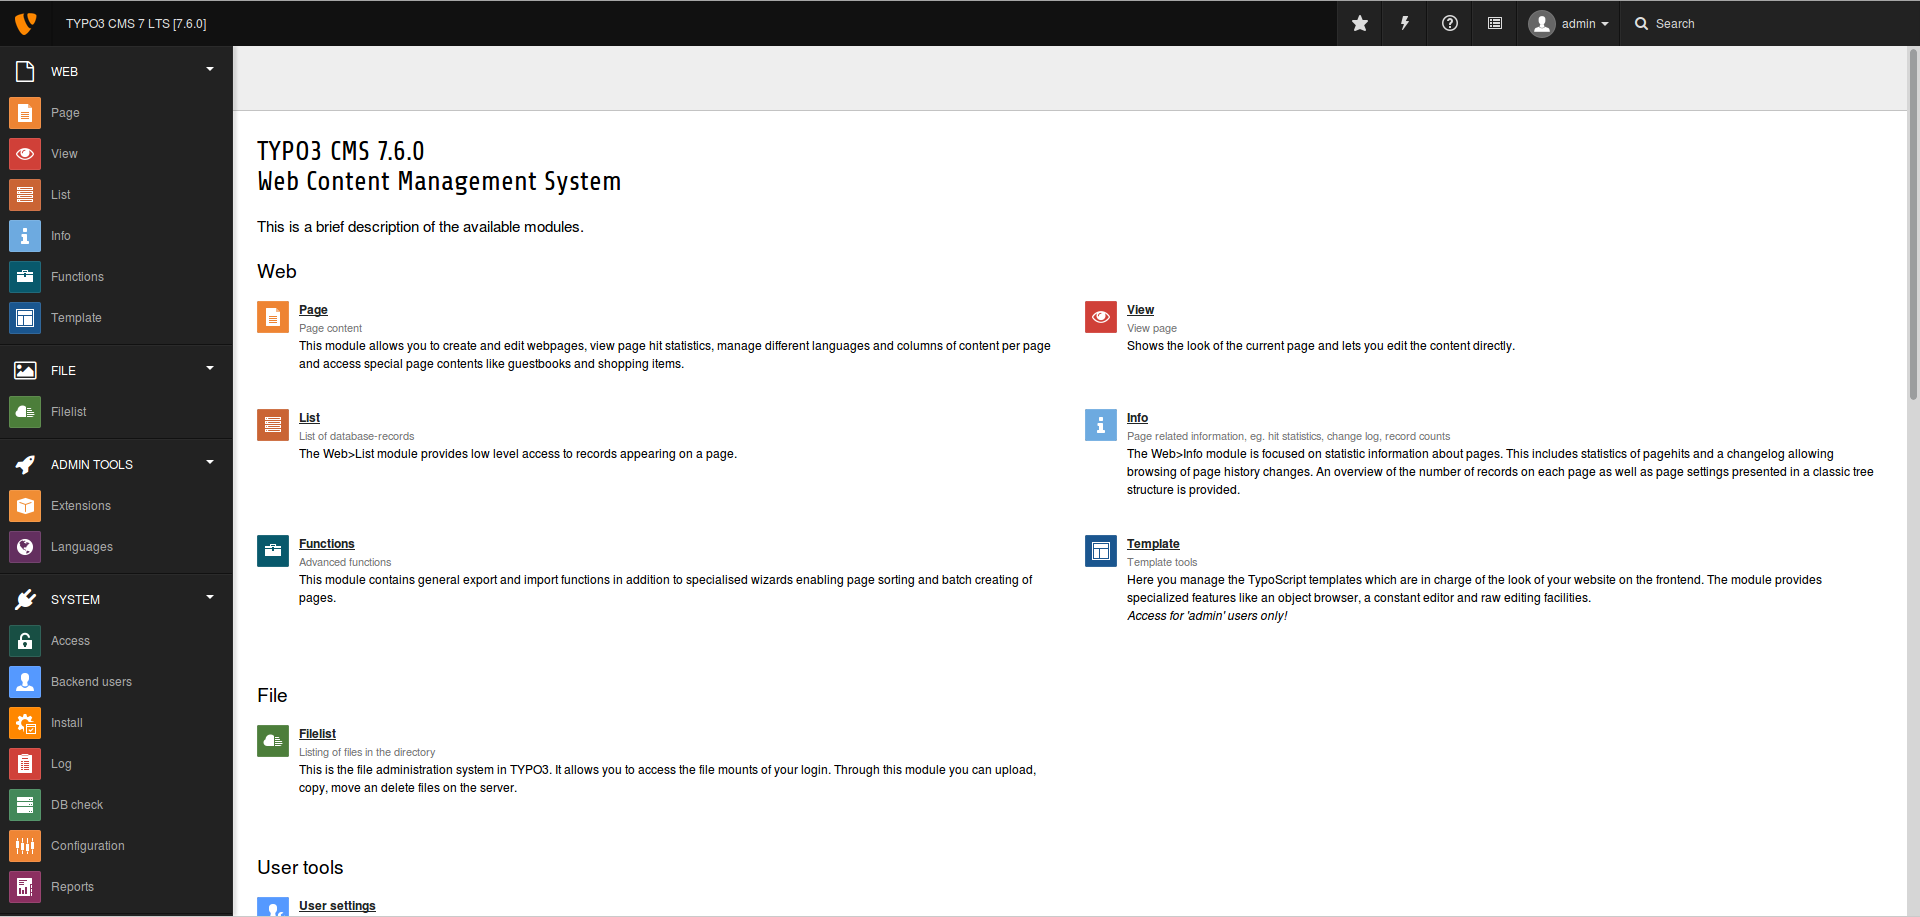
\includegraphics[width=0.90\linewidth]{BackendUserInterface/be-totalscreenshot1.png}
	\end{figure}

\end{frame}

% ------------------------------------------------------------------------------
% LTXE-SLIDE-START
% LTXE-SLIDE-UID:		f5d8b7e3-3440f409-f6d01454-4b2078a5
% LTXE-SLIDE-ORIGIN:	250b123b-2c0bfce4-506f16b0-629baa10 English
% LTXE-SLIDE-TITLE:		Look & Feel (2)
% ------------------------------------------------------------------------------

\begin{frame}[fragile]
	\frametitle{Interfaccia utente Backend}
	\framesubtitle{Look \& Feel}

	\begin{figure}
		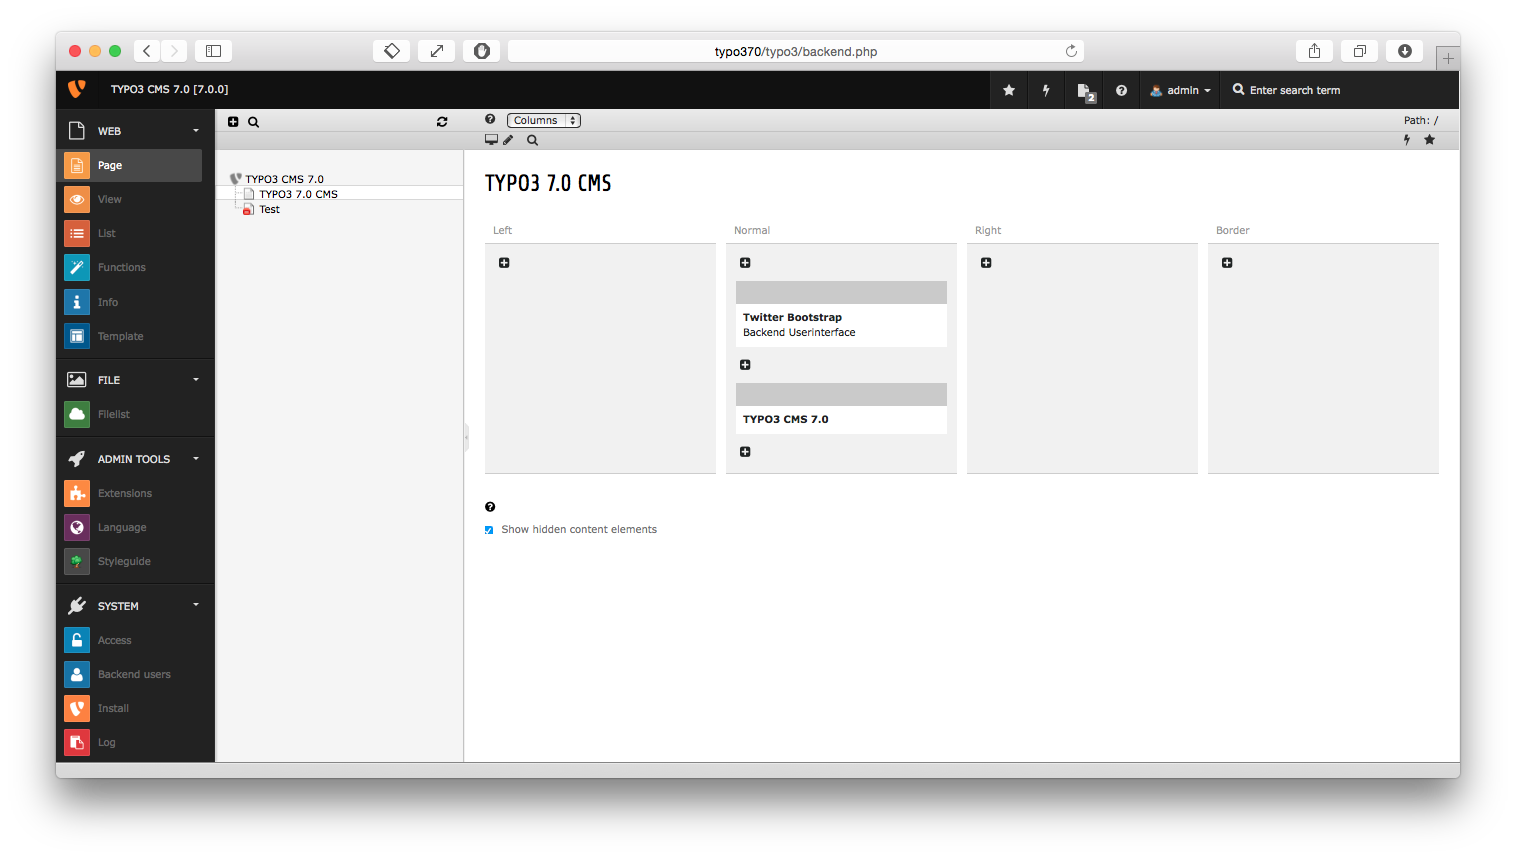
\includegraphics[width=0.90\linewidth]{BackendUserInterface/be-totalscreenshot2.png}
	\end{figure}

\end{frame}

% ------------------------------------------------------------------------------
% LTXE-SLIDE-START
% LTXE-SLIDE-UID:		4c6bf17e-c3ef47ad-23031ec4-d259ab78
% LTXE-SLIDE-ORIGIN:	2d4d33ee-071ae6ed-9f4d0c04-49361364 English
% LTXE-SLIDE-TITLE:		Look & Feel (3)
% ------------------------------------------------------------------------------

\begin{frame}[fragile]
	\frametitle{Interfaccia utente Backend}
	\framesubtitle{Look \& Feel}

	\begin{figure}
		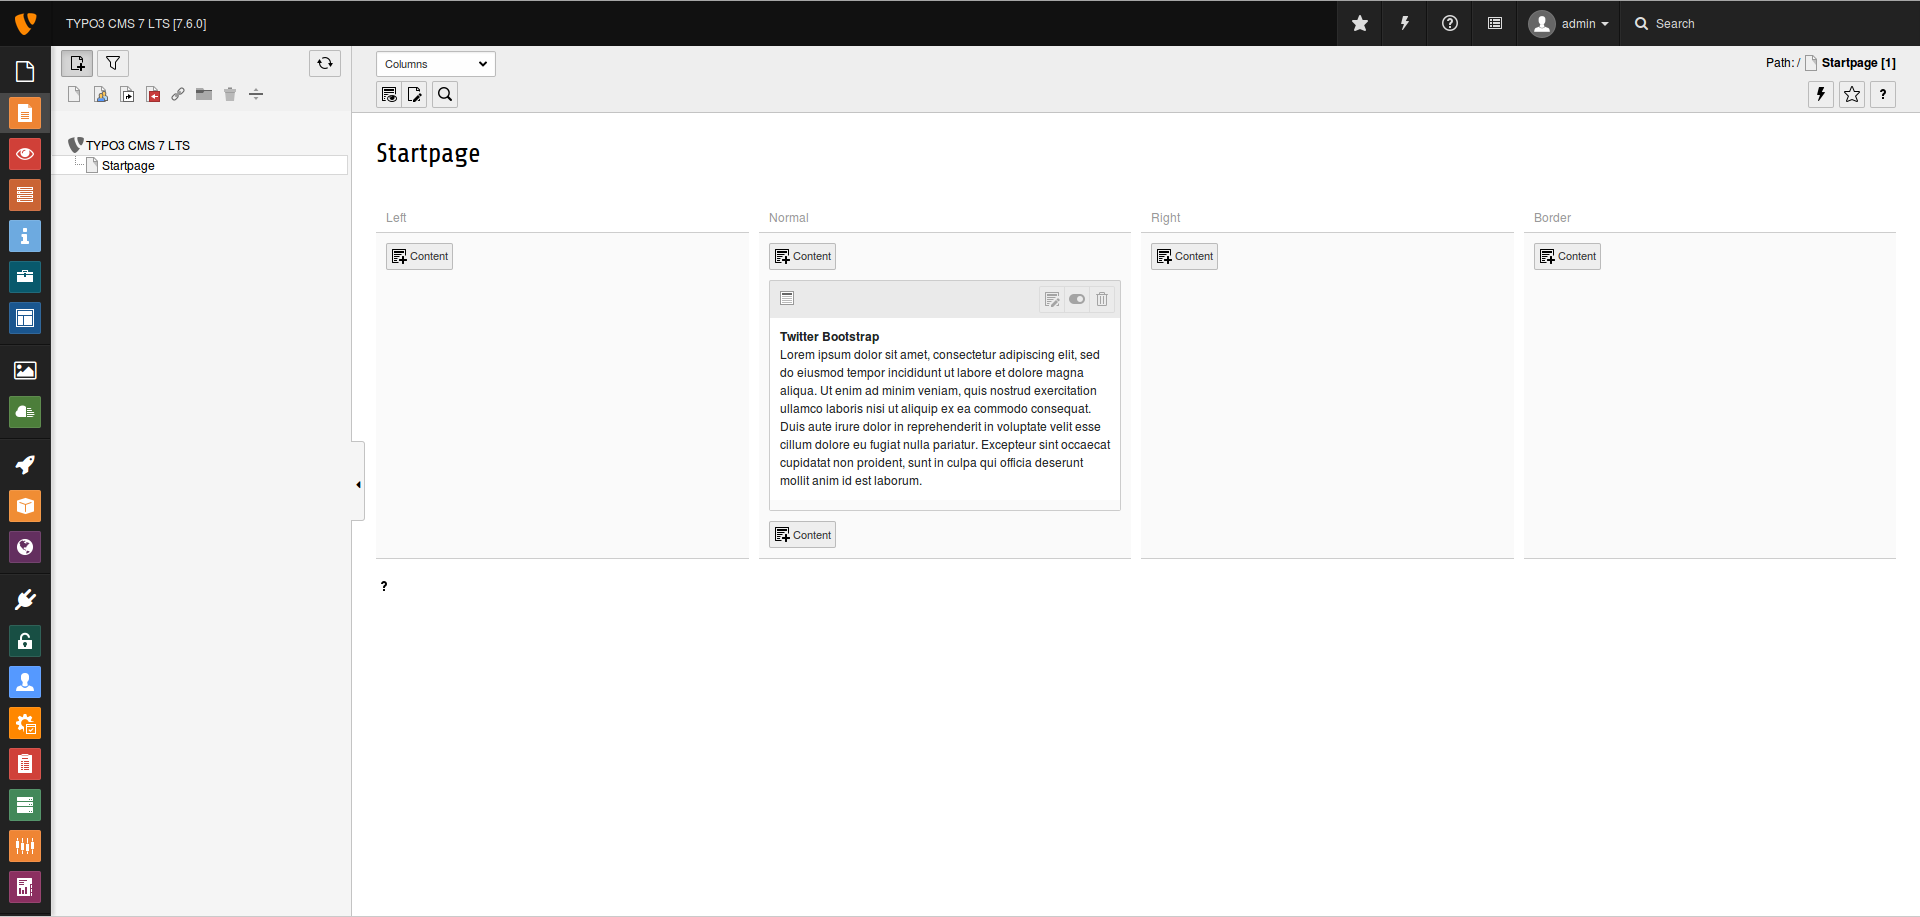
\includegraphics[width=0.90\linewidth]{BackendUserInterface/be-totalscreenshot3.png}
	\end{figure}

\end{frame}

% ------------------------------------------------------------------------------
% LTXE-SLIDE-START
% LTXE-SLIDE-UID:		c8ff3f5f-c40bd60b-84284648-08c2d3e0
% LTXE-SLIDE-ORIGIN:	de58d070-98483f3d-0949f2d1-856a9e7e English
% LTXE-SLIDE-TITLE:		Backend User Login
% ------------------------------------------------------------------------------

\begin{frame}[fragile]
	\frametitle{Interfaccia utente Backend}
	\framesubtitle{Backend User Login}

	\begin{figure}
		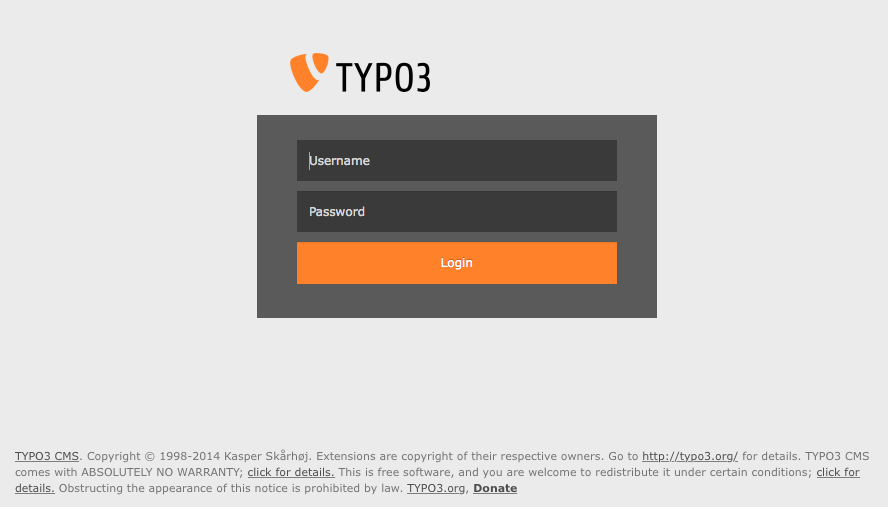
\includegraphics[width=0.80\linewidth]{BackendUserInterface/be-login.png}
	\end{figure}

\end{frame}

% ------------------------------------------------------------------------------
% LTXE-SLIDE-START
% LTXE-SLIDE-UID:		a0065935-7c1fd61f-f0e6fe80-353854ec
% LTXE-SLIDE-ORIGIN:	9baa13c8-78b2f416-28da8e3d-b234e7dc English
% LTXE-SLIDE-TITLE:		Refactor & recolor Modul Menu (Bootstrap)
% LTXE-SLIDE-REFERENCE:	https://forge.typo3.org/issues/62353
% ------------------------------------------------------------------------------

\begin{frame}[fragile]
	\frametitle{Interfaccia utente Backend}
	\framesubtitle{Top Bar (Module Menu)}

	\begin{figure}
		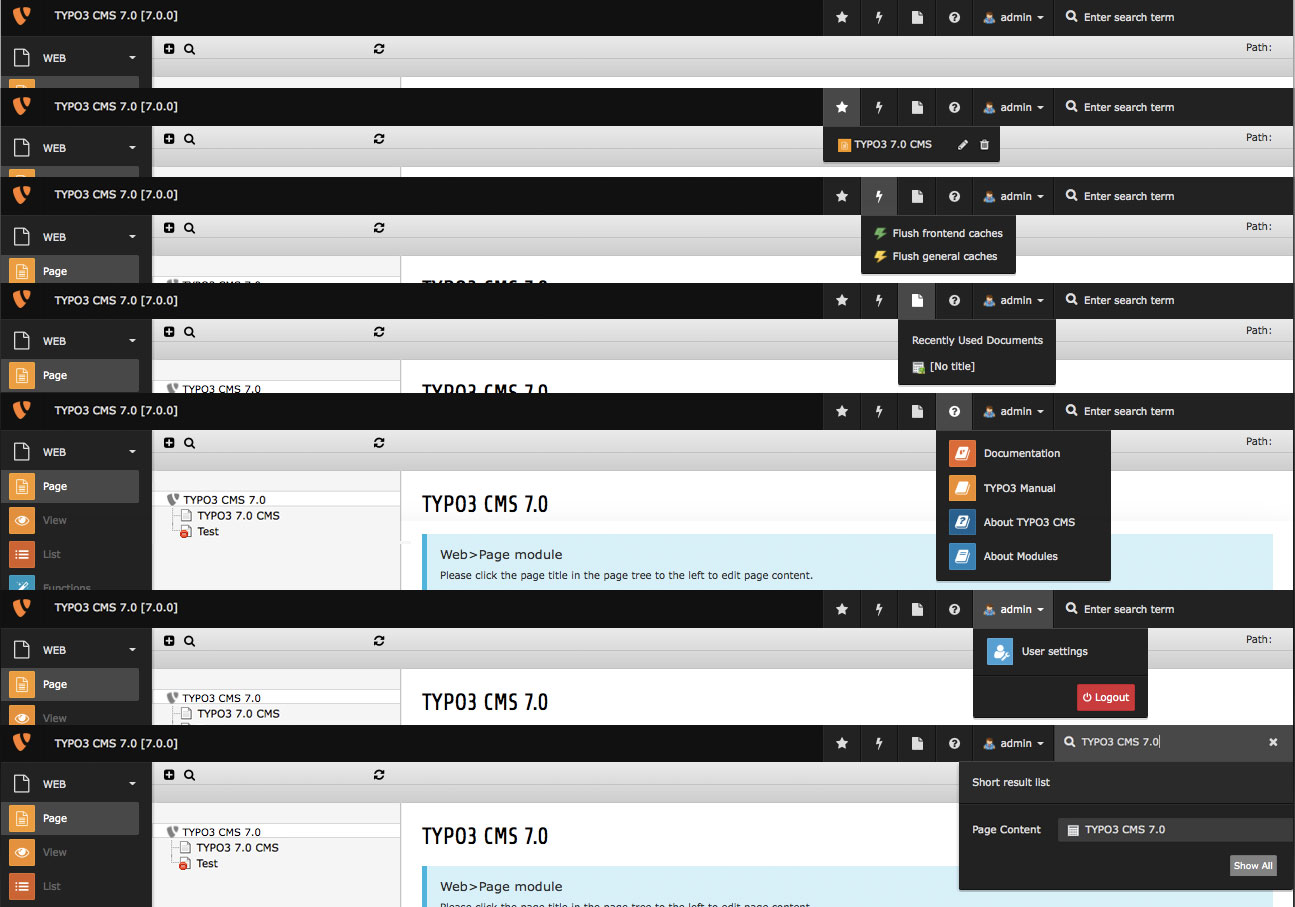
\includegraphics[width=0.70\linewidth]{BackendUserInterface/be-topbar.jpg}
	\end{figure}

\end{frame}

% ------------------------------------------------------------------------------
% LTXE-SLIDE-START
% LTXE-SLIDE-UID:		1997ccd4-42dbe12e-77b2fb67-cdb10417
% LTXE-SLIDE-ORIGIN:	4369ae5e-948d1afa-8212cd72-c91c660b English
% LTXE-SLIDE-TITLE:		New List Module Styling
% LTXE-SLIDE-REFERENCE:	https://forge.typo3.org/issues/62963
% ------------------------------------------------------------------------------

\begin{frame}[fragile]
	\frametitle{Interfaccia utente Backend}
	\framesubtitle{Modalità lista e Clipboard}

	\begin{figure}
		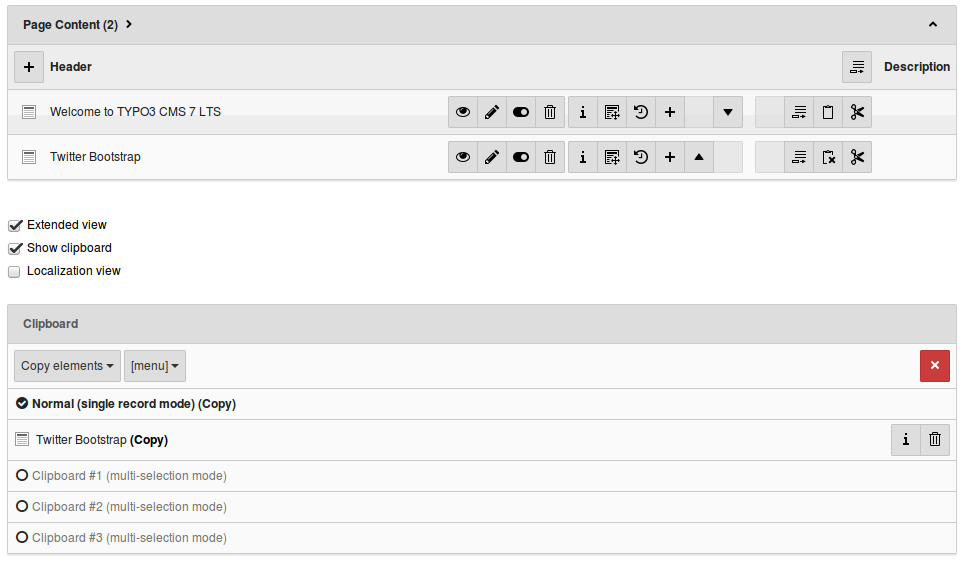
\includegraphics[width=0.80\linewidth]{BackendUserInterface/be-list.png}
	\end{figure}

\end{frame}

% ------------------------------------------------------------------------------
% LTXE-SLIDE-START
% LTXE-SLIDE-UID:		78e32ebe-885bc9ef-d5ae5891-fa061c21
% LTXE-SLIDE-ORIGIN:	252361f7-e5c42ec2-a90ecd64-4331f02b English
% LTXE-SLIDE-TITLE:		Table Style
% LTXE-SLIDE-REFERENCE:	https://forge.typo3.org/issues/62159
% ------------------------------------------------------------------------------

\begin{frame}[fragile]
	\frametitle{Interfaccia utente Backend}
	\framesubtitle{Stile tabella}

	\begin{figure}
		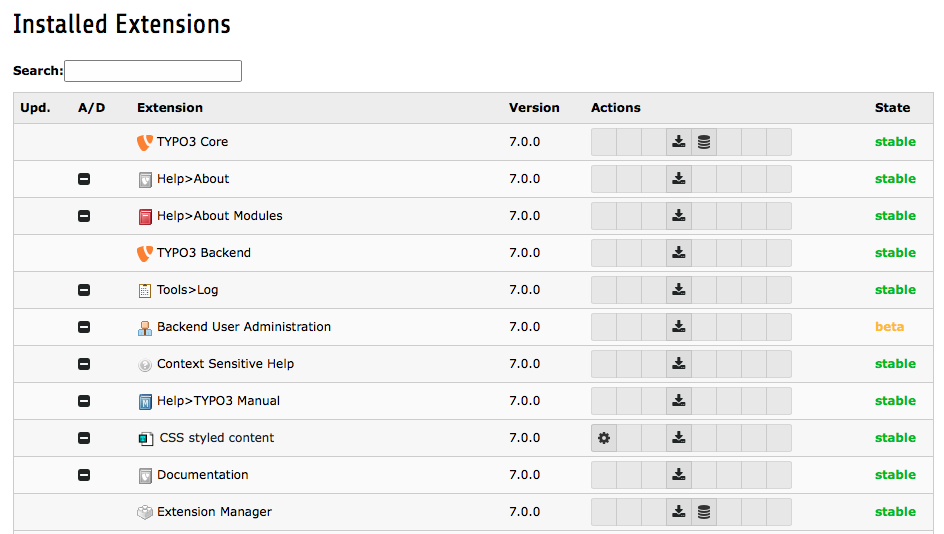
\includegraphics[width=0.99\linewidth]{BackendUserInterface/be-table.png}
	\end{figure}

\end{frame}

% ------------------------------------------------------------------------------
% LTXE-SLIDE-START
% LTXE-SLIDE-UID:		4dcd5abb-8f905c3d-0ab7e412-af49ca9d
% LTXE-SLIDE-ORIGIN:	785f717d-a7c4d1dd-f186ca6a-060c1dc4 English
% LTXE-SLIDE-TITLE:		Page And List Search
% LTXE-SLIDE-REFERENCE:	https://forge.typo3.org/issues/59763
% ------------------------------------------------------------------------------

\begin{frame}[fragile]
	\frametitle{Interfaccia utente Backend}
	\framesubtitle{Ricerca in modalità lista e pagina}

	\begin{itemize}
		\item Clicca sulla lente d'ingrandimento per vedere la barra di ricerca in modalità "lista" e "pagina"\newline
			(la funzionalità di ricerca era in fondo alla pagina prima)
	\end{itemize}

	\begin{figure}
		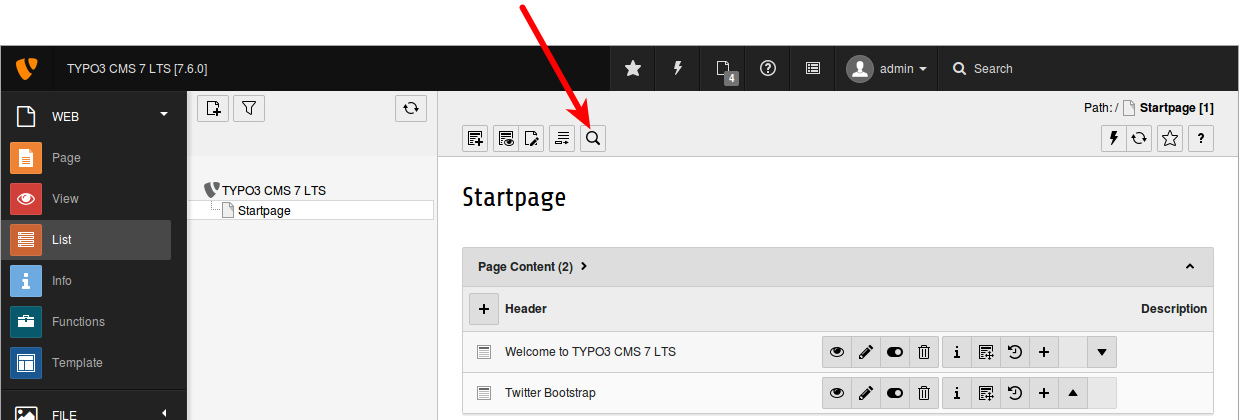
\includegraphics[width=0.95\linewidth]{BackendUserInterface/be-search.jpg}
	\end{figure}

\end{frame}

% ------------------------------------------------------------------------------
% LTXE-SLIDE-START
% LTXE-SLIDE-UID:		bb3b5ab2-57ae1361-04cde80c-47ace048
% LTXE-SLIDE-ORIGIN:	df97fbbf-9ea6c6a9-d9b4c5d4-f8fe1601 English
% LTXE-SLIDE-TITLE:		Migrate Counter of Open Documents to Bootstrap "Badge"
% LTXE-SLIDE-REFERENCE:	https://forge.typo3.org/issues/61675
% ------------------------------------------------------------------------------

\begin{frame}[fragile]
	\frametitle{Interfaccia utente Backend}
	\framesubtitle{Badge per mostrare i documenti aperti}

	\begin{itemize}
		\item Il numero di documenti aperti è mostrato come un "badge" Bootstrap\newline
			(richiede l'estensione di sistema "Open Documents")
	\end{itemize}
	\begin{figure}
		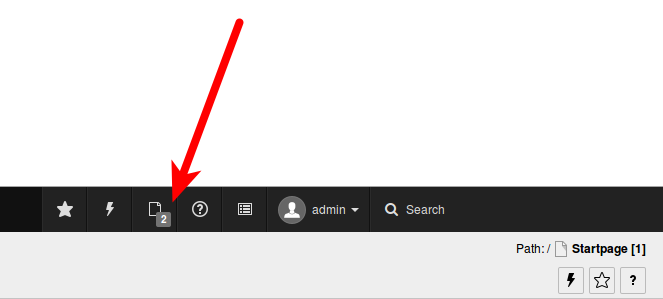
\includegraphics[width=0.75\linewidth]{BackendUserInterface/be-badge.png}
	\end{figure}

\end{frame}

% ------------------------------------------------------------------------------
% LTXE-SLIDE-START
% LTXE-SLIDE-UID:		af1f0e09-fe29c2cc-62c62205-0830e0a8
% LTXE-SLIDE-ORIGIN:	a25faae4-8c12c45e-b337b64a-0cf2f53f English
% LTXE-SLIDE-TITLE:		Rebrush FlashMessage
% LTXE-SLIDE-REFERENCE:	https://forge.typo3.org/issues/62580
% ------------------------------------------------------------------------------

\begin{frame}[fragile]
	\frametitle{Interfaccia utente Backend}
	\framesubtitle{Messaggi Flash}

	\begin{itemize}
		\item L'aspetto visivo dei messaggi Flash è stato aggiornato
		\item Migliorato il contrasto tra il testo e il colore di sfondo
	\end{itemize}

	\begin{columns}[T]
		\begin{column}{.25\textwidth}
			\smaller\hfill 
				\begingroup\color{typo3red}TYPO3 CMS < 7.0\endgroup
			\normalsize
		\end{column}

		\begin{column}{.5\textwidth}
			\begin{figure}\vspace*{-0.6cm}
				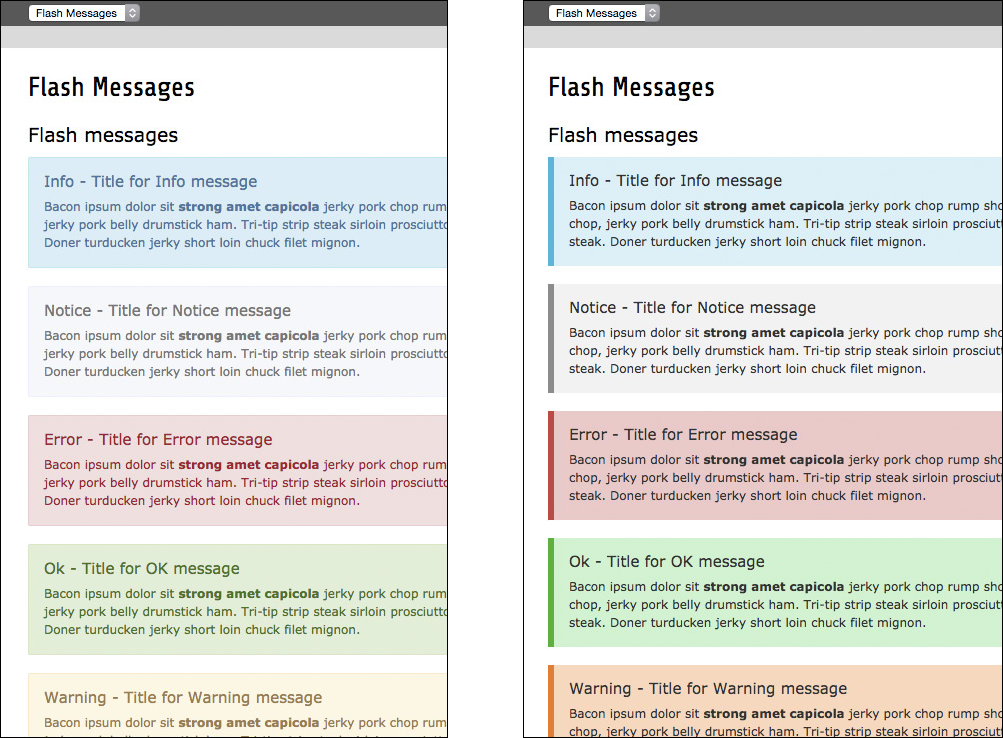
\includegraphics[width=0.99\linewidth]{BackendUserInterface/be-flashmessages.png}
			\end{figure}
		\end{column}

		\begin{column}{.25\textwidth}
			\smaller
				\begingroup\color{typo3red}TYPO3 CMS >= 7.0\endgroup
			\normalsize
		\end{column}

	\end{columns}

\end{frame}

% ------------------------------------------------------------------------------
% LTXE-SLIDE-START
% LTXE-SLIDE-UID:		879aaf99-06d28642-92a1800c-66dd0bd4
% LTXE-SLIDE-ORIGIN:	d6a85376-8109aa8c-45a40582-7edb975a English
% LTXE-SLIDE-TITLE:		Video Player in Info Window
% LTXE-SLIDE-REFERENCE:	https://forge.typo3.org/issues/61668
% ------------------------------------------------------------------------------

\begin{frame}[fragile]
	\frametitle{Interfaccia utente Backend}
	\framesubtitle{Video Player nella finestra delle informazioni}
	\begin{itemize}
		\item I file HTML5 audio e video possono essere eseguiti nella finestra delle informazioni 
			(dove sono mostrati i meta data)
		\begin{figure}
			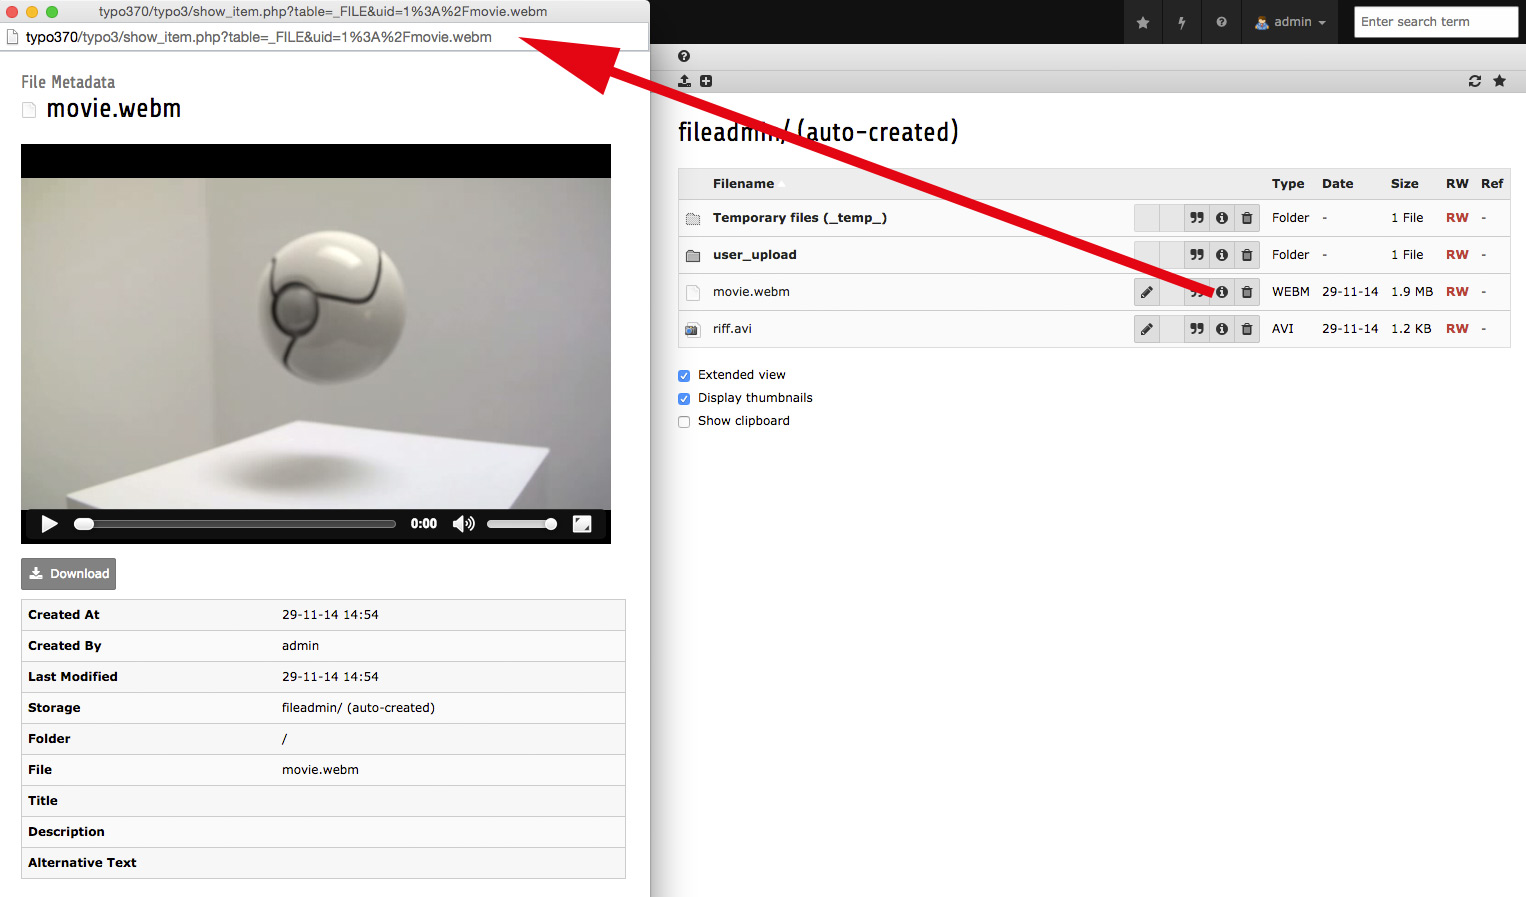
\includegraphics[width=0.70\linewidth]{BackendUserInterface/be-info.jpg}
		\end{figure}

	\end{itemize}

\end{frame}

% ------------------------------------------------------------------------------
